\documentclass{article}
%\usepackage{arxiv}
%\usepackage[T1,T2A]{fontenc}

\usepackage[utf8]{inputenc}
\usepackage[english]{babel}
\usepackage{url}
\usepackage{booktabs}
\usepackage{amsfonts}
\usepackage{nicefrac}
\usepackage{microtype}
\usepackage{lipsum}
\usepackage{graphicx}
\usepackage{doi}
\newtheorem{theorem}{Theorem}
\newtheorem{lemma}[theorem]{Lemma}

\usepackage[utf8]{inputenc}
\usepackage{amsmath}
\usepackage{mathtools}

\usepackage{algorithm}
\usepackage{algpseudocode}

\usepackage{babel,csquotes,newcent,textcomp}
\usepackage[backend=biber,sortcites]{biblatex}


\usepackage{lipsum}
\title{Stochastic Newton with Arbitrary Sampling}

\author{ Igor ~Melnikov	\\
	Moscow Institute of Physics and Technology\\
	Dolgoprudny, Russia \\
	\texttt{melnikov.ia@phystech.edu} \\
	%% examples of more authors
	\and
	Rustem Islamov \\
	Institut Polytechnique de Paris\\
	Palaiseau, France \\
	\texttt{rustem.islamov@ip-paris.fr} \\
}

\addbibresource{mybib.bib}
\begin{document}
\maketitle

\begin{abstract}
We analyse stochastic Newton-type methods for solving Empirical Risk Minimization problem. We prove fast local convergence rates independent of the condition number. Unlike most other stochastic variants of second order methods, which require the evaluation of a large number of gradients and/or Hessians in each iteration to guarantee convergence, the method do not have this shortcoming. We investigate the performance of the method by applying existing sampling strategies.
\end{abstract}

\section{Introduction}
\begin{equation}\label{eq:problem}
    \min\limits_{x\in \mathbb{R}^d} \left[f\left(x\right):=\cfrac{1}{n}\sum\limits_{i=1}^{n}f_i\left(x\right)\right].
\end{equation}
Here $n$ is the number of data points that is typically extremely large in real problems; $d$ is the number of model parameters. Ususally, $f_i$ denotes the value of a loss function on $i$-th data point $(a_i, b_i)$. One of the examples of the problem that has the form of \eqref{eq:problem} is Logistic Regression problem where
\begin{equation}
    f_i(x) = \log\left(1+\exp(-b_i a_i^\top x )\right),
\end{equation}
where $a_i \in \mathbb{R}^d$ and $b_i \in \{-1,1\}.$

As $n$ is large the problem~\eqref{eq:problem} is typically solved by First-order methods that uses only one data point per iteration. These methods are extensively studied \cite{litlink1} and there are a wide variety of variations of such techniques. In particular, the Stochastic Gradient Descent(SGD) is often used, the distinguishing feature of which is cheap iterations independent of $n$. Nevertheless, SGD with constant-stepsize has a number of disadvantages, the main of which is that it converges only up to the neighbourhood of the solution, not the exact solution. This problem arises since stochastic gradient estimator has non-zero variance. Radius of this convergence area is proportional to the variance of the stochastic gradient. The so-called variance-reduced methods \cite{svrg, saga} are used to solve this problem. They have the same iteration cost as SGD, but now the algorithm converges to the exact solution. However, all first-order methods known to us are characterized by the dependence of the required number of iterations on the condition number\footnote{For a continuously Differentiable function $f$ condition number is defined as $\lim\limits_{\varepsilon \rightarrow 0} \sup\limits_{\left\|\partial x\right\| \leq \varepsilon} \frac{\left\|\partial f\left(x\right)\right\|}{\left\|\partial x\right\|}$,\\ for $L$-smooth and $\mu$-convex function the condition number is $\frac{L}{\mu}$}. This makes impossible using SGD and its variants for ill-conditioned problems.

In classic optimization one of the solutions is to use second-order information about the objective. Classic Newton's method adapts to the curvature of the problem and thereby decrease the dependence on the condition number. The step of Newton's method has the following form

\begin{equation}
    x^{k+1} = x^k - \left(\nabla^2f\left(x^k\right)\right)^{-1}\nabla f\left(x^k\right)
\end{equation}

In the case of ERM we need to compute $n$ Hessians per iteration which is extremely costly in practice. Our desire is to use only a few Hessians in each iteration. One of the most popular directions is so called Subsampled Stochastic Newton's methods \cite{litlink7}. Despite first-order methods, these methods are poorly understood, and the theory usually requires a large batch sizes. To the best of our knowledge there are just a few works that provable work with arbitrary batch sizes \cite{litlink3, litlink5, litlink6}.

In this work we focus on the Algorith 1 of  \cite{litlink4}. They presentes the following algorithm:

\begin{algorithm}\label{eq:algorithm}
\caption{Stochastic Newton (SN)}\label{alg:cap}
\begin{algorithmic}
\State {$\textbf{Initialize:}$ Choose starting iterates $w_1^0, w_2a^0, \dots, w_n^0 \in \mathbb{R}^d$ and minibatch size $\tau \in \{1, 2, \dots, n\}$}
\For {$k = 1, \dots$}
    \State {$x^{k+1} = \left(\sum\limits_{i=1}^n\nabla^2f_i\left(w_i^k\right)\right)^{-1}\sum\limits_{i=1}^n \left(\nabla^2f_i\left(x^k\right)w_i^k - \nabla f_i\left(w_i^k\right)\right)$}
    \State {Choose a subset $k \subseteq \{1,\dots, n\}$ of size $\tau$ uniformly at random}
    \State {
        $w_i^{t+1}= 
    \begin{cases}
        w_i^{t} &i \not\in S^t\\
        x^{t + 1} &i \in S^t\\
     \end{cases}$
}
\EndFor
\end{algorithmic}
\end{algorithm}


% \begin{equation*}
% \begin{multlined}
% w^0_i = x^0 \text{, for } i \in \overline{1, n}. \\
% w_i^{t+1}= 
%  \begin{cases}
%   w_i^{t} &i \not\in S^t\\
%   x^{t + 1} &i \in S^t\\
%  \end{cases}
%  \end{multlined}
% \end{equation*}
% $S^k$ is uniformly chosen random subset of $\{1, \dots, n\}$ with size $\tau$. \\

% The algorithms looks the following way:

% \begin{equation}
% \begin{multlined}
%     x^{k+1} = \left(\sum\limits_{i=1}^n\nabla^2f_i\left(w_i^k\right)\right)^{-1}\sum\limits_{i=1}^n \left(\nabla^2f_i\left(x^k\right)w_i^k - \nabla f_i\left(w_i^k\right)\right)
% \end{multlined}
% \end{equation}

We investigate how the sampling strategies affect the performance of Algorithm \eqref{eq:algorithm}. In practice, the uniform sampling is not the best choice, and we need to use another strategies how to choose a set $S^t$. 

\section{Problem Statement}

Assume we have $n$ training points $\left(a_i, b_i\right)$ for $i \in \overline{1, n}$. We also assume $n$ to be large. Let $f_i\left(x\right)$ be a loss function on $i$-th training point . We analyze second order methods solving Empirical Risk Minimization problem of the form.

One of the examples of the problem that has the form of \eqref{eq:problem} is Logistic Regression problem where
\begin{equation}
    f_i(x) = \log\left(1+\exp(-b_i a_i^\top x )\right),
\end{equation}
where $a_i \in \mathbb{R}^d$ and $b_i \in \{-1,1\}.$


\begin{equation}
    \min\limits_{x\in R} \left[f\left(x\right):=\cfrac{1}{n}\sum\limits_{i=1}^{n}f_i\left(x\right)\right].
\end{equation}

\section{Experiment Plan}

The experiment applies Algorithm 1 to minimize the logistic regression risk function with $l_2$ regularization.

\begin{equation}
    f_i(x) = \log\left(1+\exp(-b_i a_i^\top x )\right) + \frac{\lambda}{2}\|x\|,
\end{equation}

The main experiment is to establish the dependence of convergence accuracy on the size of the batch. The goal is to establish that conditional number does not significantly affect convergence. To do this, it is sufficient to establish that the curves are not very different. 

We generate the synthetic data by the make classification function of the scikit-learn library, where n = 500 and d = 5. Each row of the data matrix is normalized such that $\|a_i\| = 1$. We run experiments for $\lambda = \{10^{-1}, 10^{-3}, 10^{-4}\}$, which leads to conditional number differ more than in 10 times.
Initial point $x^0$ is taken as the result of GD in 30 iteration.

\newpage

We expect table in presented as pandas.DataFrame with columns=['k(iter num)', 'Ak/A0', 'tau', 'lambda'].

Expected plots.\\  
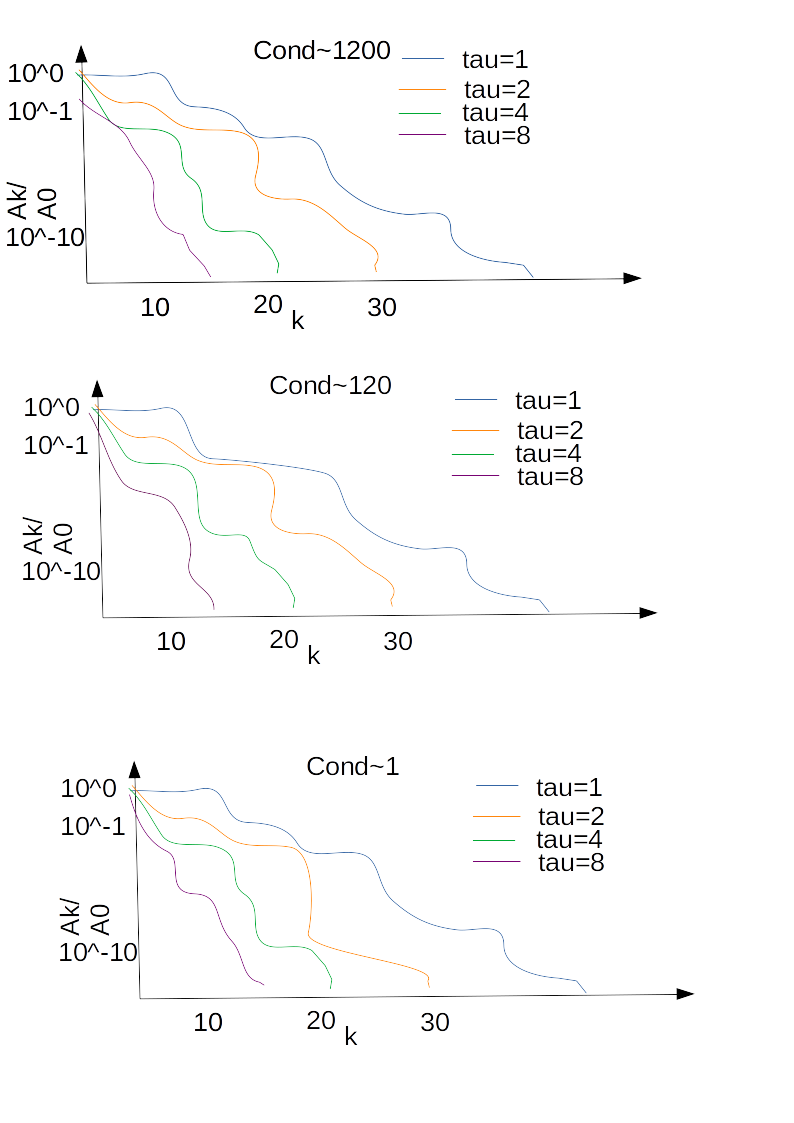
\includegraphics[width=90mm]{sketch.png}

x-axis is number of iterations of the algorithm. y-axis is ratio $\cfrac{A_0}{A_k}$,where $A_0 = |x^*-x^0|, A_k = |x^*-x^k|$.

\section{Preliminary report}
Convergence has been established. For lambdas 0.001 and 0.0001 the difference in accuracy at 100th iteration is less than in 1.2 times for all butch sizes. However for lambda 0.1 accuracy is much higher - that is a fact to investigate in more detail.

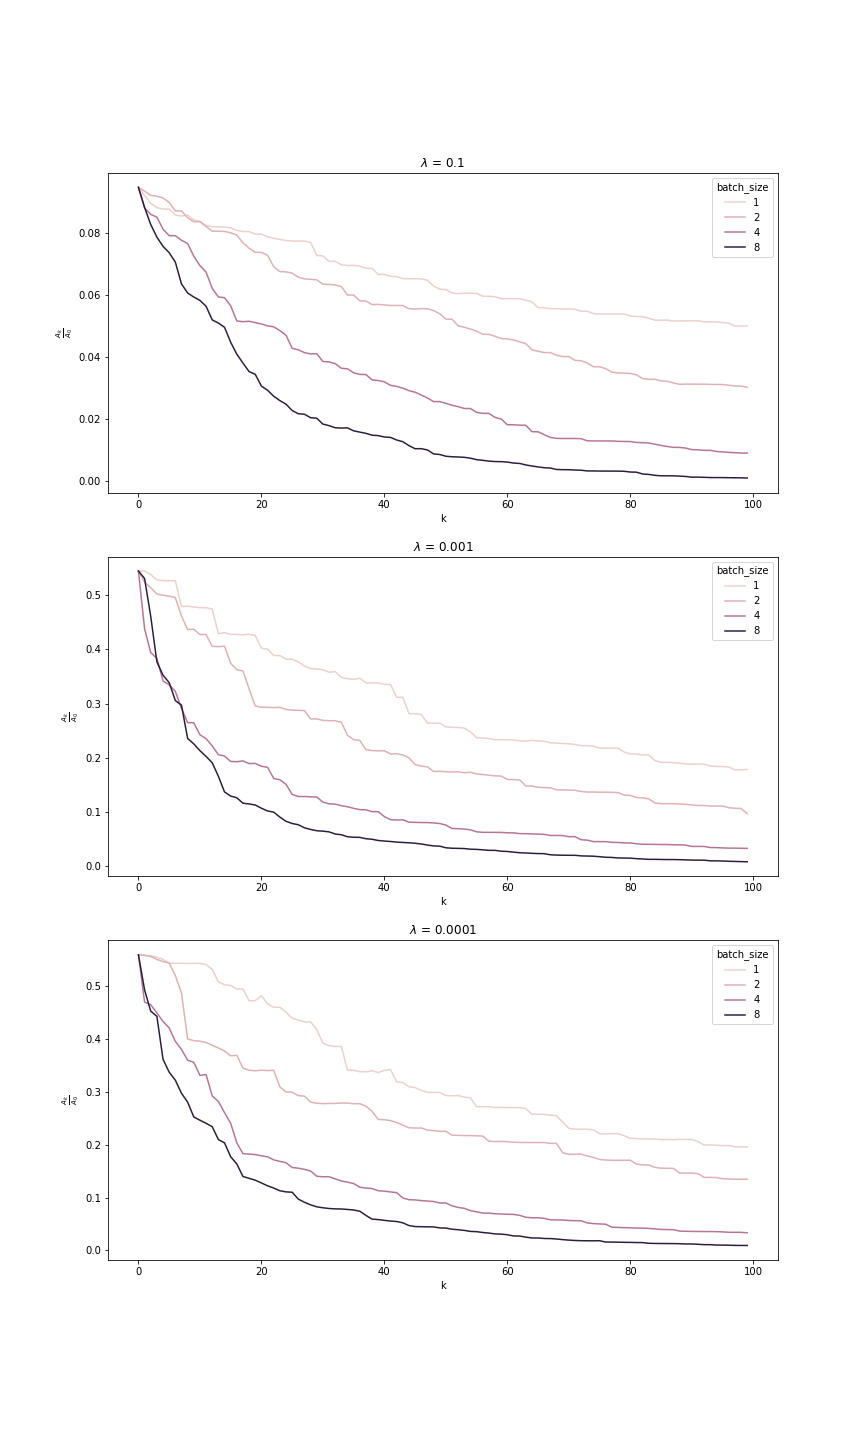
\includegraphics[width=90mm]{plot.png}

\section{Run Basic Code}
We have implemented algorithm 1. 

Competitive models for our algorithm were described in Introduction section with links on description. These models are  Gradient Descent, Stochastic Gradient Descent, variance-reduced methods, classical Newton's method.

A description of the algorithm in the form of pseudocode is given in the introduction.
\section{Theoretical part}

The proof was based on the proof in the article 1.

\begin{theorem} Assume that every $f_i$ is $µ$-strongly convex and has $H$-Lipschitz Hessian and consider
the following Lyapunov function:
\begin{equation}
    W^k \overset{def}{=} \frac{1}{n}\sum\limits_{i=1}^{n}\|w_i^k - x^\star\|.
\end{equation}

Then for the random iterates of NS Algorithm we have the recursion:
\begin{equation}
    \mathbf{E}_k W^{k + 1} \leq \left(1 - \frac{\tau}{n} +
    \frac{\tau}{n}\left(\frac{H}{2\mu}\right)^2W^k\right)W^k.
\end{equation}

Furthermore if $\|w_i^0 - x^\star\| \leq \frac{\mu}{H}$, for $i \in \{1, \dots, n\}$ and $\min_{i \in \{1, \dots, n\}}{p_i} \geq \frac{\tau}{4n}$, then
\begin{equation}
    \mathbf{E}_k W^{k + 1} \leq \left(1 - \frac{3\tau}{4n}\right)W^k.
\end{equation}
\end{theorem}

This theorem implies at least linear convergence rate for all $\tau$ in our algorithm.
Let's denote by $p_i$ probability of i be in $S$. $|sum|limits_{i=1}^n p_i = \tau$

\begin{lemma} (taken from article 1.).
Let $f_i$ be $\mu$-strongly convex and have $H$-Lipschitz Hessian for all $i = 1, \dots, n$. Then
the iterates of the Algorithm satisfy:
\begin{equation}
    \|x^k - x^\star\| \leq \frac{H}{2\mu}W^k.
\end{equation}
\end{lemma}

\begin{lemma}
If $\|w_i^0 - x^\star\| \leq \frac{\mu}{H}$, for $i \in \{1, \dots, n\}$, then for all $k$, for $i \in \{1, \dots, n\}$
\begin{equation}
    \|w_i^k - x^\star\|^2 \leq \left(\frac{\mu}{H}\right)^2
\end{equation}
\end{lemma}

\begin{lemma} The random iterates of the Algorithms satisfy the identity
\end{lemma}
Proof:
\begin{equation*}
\begin{split}
    \mathbf{E}_k W^{k + 1} = \frac{1}{n}\sum\limits_{i=1}^{n}\mathbf{E}_k\|w_i^{k + 1} - x^\star\| =
     \frac{1}{n}\sum\limits_{i=1}^{n}p_i\|x^k - x^\star\| + \frac{1}{n}\sum\limits_{i=1}^{n}(1 - p_i)\|w_i^k - x^\star\| = \\
     \frac{\tau}{n}\|x^k - x^\star\| + \frac{1}{n}\sum\limits_{i=1}^{n}(1 - p_i)\|w_i^k - x^\star\| \leq
     \frac{\tau}{n}\left(\frac{H}{2\mu}\right)^2\left(W^k\right)^2 + \frac{1}{n}\sum\limits_{i=1}^{n}(1 - p_i)\|w_i^k - x^\star\| \leq \\
     \frac{1}{4}\frac{\tau}{n}W^k + \frac{1}{n}\sum\limits_{i=1}^{n}(1 - p_i)\|w_i^k - x^\star\| \leq \frac{1}{4}\frac{\tau}{n}W^k + \frac{1}{n}(1 - \min_{i \in \{1, \dots, n\}}{p_i})\sum\limits_{i=1}^{n}\|w_i^k - x^\star\|  = \\ \frac{1}{4}\frac{\tau}{n}W^k + (1 - \min_{i \in \{1, \dots, n\}}{p_i})W^k =  \left(\frac{1}{4}\frac{\tau}{n} + 1 - \min_{i \in \{1, \dots, n\}}{p_i}\right)W^k.
\end{split}
\end{equation*}

\newpage
\addcontentsline{toc}{section}{Список используемой литературы}

%далее сам список используевой литературы
\printbibliography
\end{document}


